\begin{figure}[t]
\centering
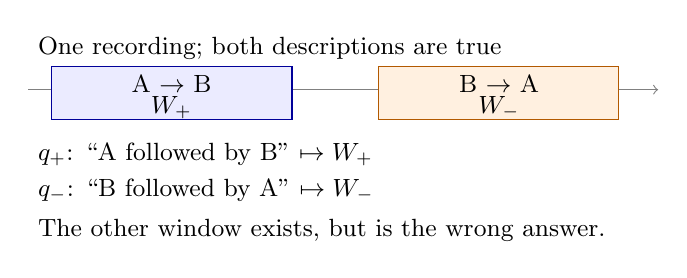
\begin{tikzpicture}[x=1cm,y=1cm,every node/.style={font=\small}]
\node[anchor=west] at (0,1.93) {One recording; both descriptions are true};
\draw[->,gray] (0,1.4)--(8.0,1.4);
\draw[fill=blue!8,draw=blue!60!black] (.3,1.02) rectangle (3.35,1.7);
\draw[fill=orange!12,draw=orange!70!black] (4.45,1.02) rectangle (7.5,1.7);
\node at (1.82,1.47) {A $\rightarrow$ B};
\node at (5.98,1.47) {B $\rightarrow$ A};
\node at (1.82,1.17) {$W_+$};
\node at (5.98,1.17) {$W_-$};
\node[anchor=west] at (0,.58) {$q_+$: ``A followed by B'' $\mapsto W_+$};
\node[anchor=west] at (0,.12) {$q_-$: ``B followed by A'' $\mapsto W_-$};
\node[anchor=west] at (0,-.38) {The other window exists, but is the wrong answer.};
\end{tikzpicture}
\caption{RelTwin schematic, not an observed prediction. Each query sees the full audio and is contrasted against both timestamp answers. The two descriptions share event categories; their target windows differ.}
\label{fig:pair}
\end{figure}
